\chapter{中心极限定理}
\begin{introduction}
  \item Intro to Prob\quad5.4 
  \item Prob $\&$ Stat\quad4.4
\end{introduction}
\section{引导问题}
根据分布的可加性,我们知道卡方分布是具备可加性的。具体来说,若$X_i$是独立同分布的卡方分布随机变量,即$X_i \sim \chi^2(1)$。于是,
\begin{eqnarray*}
    S_{k} = \sum_{i=1}^{k}X_i \sim \chi^2(k)
\end{eqnarray*}
我们考虑1个、2个、10个以及30个随机变量之和的密度函数见图\ref{fig:lect13_sum_of_chisquared_rv}。
\begin{figure}[ht]
    \centering
    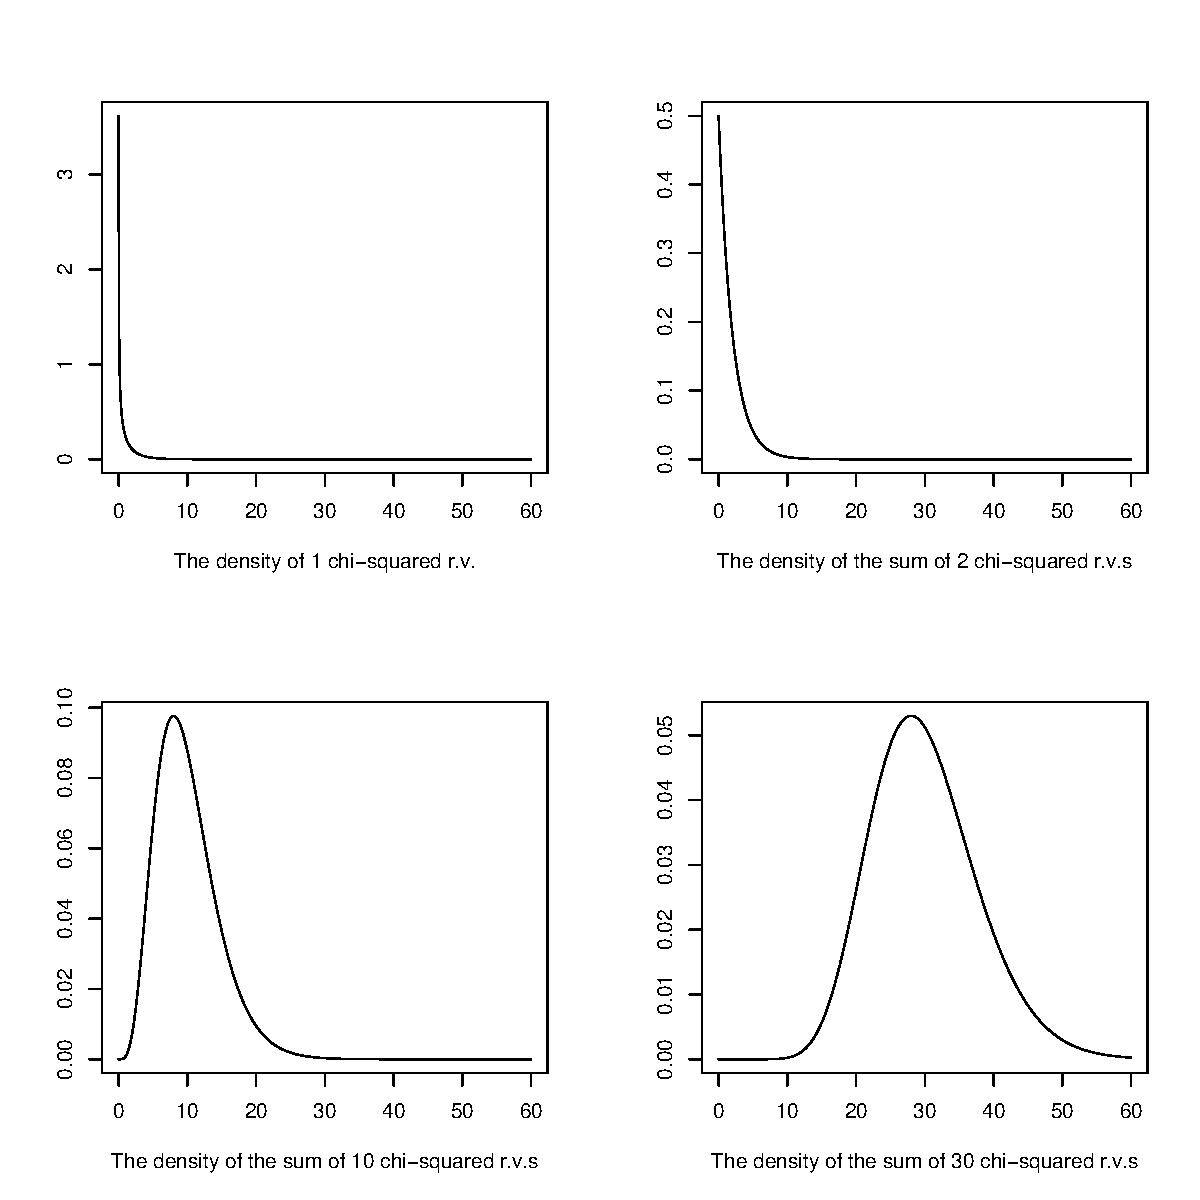
\includegraphics[scale=0.63]{image/Lect13_sum_of_chisquares.pdf}
    \caption{多个卡方分布之和的密度函数}
    \label{fig:lect13_sum_of_chisquared_rv}
\end{figure}

\begin{remark}
随着$k$的增加,$S_k$的密度函数图像越来越接近正态分布曲线。
\end{remark}

对于卡方分布$\chi^2(k)$而言,其期望和方差分别为$$
E(S_k)=k, \quad \text{Var}(S_k) = 2k.$$
当$k$增加时,$S_k$的密度函数的位置右移,且$p_{k}(s)$的方差也增大。这意味着这个分布的中心趋向$\infty$,其方差也趋向$\infty$,分布极不稳定。因此,直接讨论$S_k$的分布是有困难的。于是,在中心极限定理的研究中均对$S_k$进行标准化,即
$$
S_k^\ast = \frac{S_k - E(S_k)}{\sqrt{\text{Var}(S_k)}}
$$
可以证明
\begin{eqnarray*}
    E(S_k^\ast) = 0\\
    \text{Var}(S_k^\ast) = 1
\end{eqnarray*}
一个很自然的问题是$S_k^{\ast}$的极限分布是否为标准正态分布$N(0,1)$?
\begin{problem}
   中心极限定理本身研究的是\textbf{在什么条件下},随机变量之和的极限分布是正态分布。
\end{problem}

\section{独立同分布下的中心极限定理}
\begin{theorem}[林德伯格-莱维(Lindeberg-Levy)中心极限定理]
设$\{X_n\}$是独立同分布的随机变量序列,且$E(X_i)=\mu,\text{Var}(X_i) = \sigma^2>0$存在,若记
$$
S_n^{\ast} = \frac{\sum_{i=1}^n X_i - n \mu}{\sigma \sqrt{n}},
$$
则对任意实数$y$,有
$$
\lim_{n\rightarrow \infty} P(S_n^{\ast} \leq s) = \Phi(s)
$$
\end{theorem}
\begin{remark}
    \begin{enumerate}
        \item 这个定理的证明需要利用特征函数,学生可以参考《概率论与数理统计教程》第212页。
        \item 林德伯格-莱维中心极限定理表示独立同分布,且二阶矩存在的随机变量序列是满足中心极限定理。
    \end{enumerate}
\end{remark}

以下,我们讨论一种特定的分布——二项分布。

\begin{theorem}[棣莫弗-拉普拉斯(de Moivre-Laplace)中心极限定理]
   设 $n$重伯努利实验中,事件$A$在每次实验中出现的概率为$p(0<p<1)$,记$S_n$为$n$次实验中实验$A$出现的次数,且记
   $$
   S_n^{\ast} = \frac{S_n - np}{\sqrt{np(1-p)}}
   $$
   则对任意实数$y$,有
   $$
\lim_{n\rightarrow \infty} P(S_n^{\ast} \leq s) = \Phi(s).
   $$
\end{theorem}
\begin{remark}对于棣莫弗-拉普拉斯(de Moivre-Laplace)中心极限定理,我们具体讨论一下。
\begin{enumerate}
    \item 二项分布的近似分布,可以采用泊松分布,也可以使用正态分布。一般来说,在$p$比较小时,用泊松分布近似较好;而在$np>5$和$n(1-p)>5$时,用正态分布比较好。
    \item 因为二项分布是离散分布,而正态分布是连续分布,在近似时通常可以做一些修正来提高精度。对任意$s_1<s_2$,$P(s_1 \leq S_n \leq s_2)$的修正方案为
    $$
    P(s_1-0.5 \leq S_n \leq s_2+0.5) = \Phi\left(\frac{s_2+0.5 - np}{\sqrt{np(1-p)}}\right) - \Phi\left(\frac{s_1 - 0.5 - np}{\sqrt{np(1-p)}}\right).
    $$
    \begin{example}
        若$S_n \sim b(25,0.4)$,那么$P(5\leq S_n \leq 15) = 0.9774$。我们可以计算
        \begin{eqnarray*}
            \text{修正后:}P(5\leq S_n \leq 15) &=& \Phi\left(\frac{15+0.5 - 10}{\sqrt{25\times 0.4\times 0.6}}\right) -\Phi\left(\frac{5-0.5 - 10}{\sqrt{25\times 0.4\times0.6}}\right) = 0.9753,\\
             \text{未修正:}P(5\leq S_n \leq 15) &=& \Phi\left(\frac{15 - 10}{\sqrt{25\times 0.4\times 0.6}}\right) -\Phi\left(\frac{5 - 10}{\sqrt{25\times 0.4\times 0.6}}\right) = 0.9588.
            \end{eqnarray*}
    \end{example}
    同时,这种修正方案也可以适用于计算$P(S_n = k)$的情况。
    \begin{example}
         若$S_n \sim b(25,0.4)$,那么$P(S_n = 10) = 0.1612$。根据修正方案,我们可以计算
         $$
         \Phi\left(\frac{10+0.5 - 10}{\sqrt{25\times 0.4\times 0.6}}\right) -\Phi\left(\frac{10-0.5 - 10}{\sqrt{25\times 0.4\times 0.6}}\right) = 0.1617.
         $$
    \end{example}
\end{enumerate}
\end{remark}
\section{棣莫弗-拉普拉斯中心极限定理的应用案例}
回顾一下棣莫弗-拉普拉斯中心极限定理,我们知道
$$
P(S_n^{\ast} \leq s) = \Phi(s).
$$
注意到,$\Phi(s)$本质上是一个概率值。对于给定概率$\Phi(s)$时,$s$可以认为是相应的分位数。而二项分布中由两个参数$n$和$p$,其中$n$表示实验次数,也通常被认为是样本量(这个概念将会在第14讲中给出)。

于是,在棣莫弗-拉普拉斯中心极限定理的应用,我们要解决以下三个问题:
\begin{enumerate}
    \item 求分位数;
    \item 求概率;
    \item 求样本量。
\end{enumerate}
\subsection{求分位数}
\begin{example}
某奶茶店共售卖两种奶茶:珍珠奶茶和纯奶茶。其差异在于是否放珍珠。假设每位顾客点任何一种奶茶是等可能的,且点单是相互不受影响。已知每杯珍珠奶茶中需放入5克珍珠。请问,至少要准备多少克珍珠,才可以有$95\%$的可能性,接受100杯奶茶的点单?
\end{example}
\begin{solution}
设第$i$位顾客点了珍珠奶茶为$X_i$,$X_i \sim b(1,p_0),p_0=0.5$,即
 $$X_{i}=\left\{\begin{aligned}
 &1,&\text{如果第i位顾客点了珍珠奶茶}\\
&0,&\text{如果第i位顾客点了纯奶茶}\\
 \end{aligned}\right.$$
 所以,100位顾客中共有
 $$
 \sum_{i=1}^{100}X_i \sim b(100,p_0)
 $$
 点了珍珠奶茶。设我们拟准备$s$克珍珠。于是,$s$克珍珠能够满足100位顾客的点单,即
 \begin{eqnarray*}
      95\% &\leq& P\left(  5\times \sum_{i=1}^{100}X_i \leq s\right)\\
      & = & P\left(   \sum_{i=1}^{100}X_i \leq \frac{s}{5}\right) \\
      & = & P\left(\frac{\sum_{i=1}^{100} X_{i}-50}{\sqrt{25}} \leq \frac{\frac{s}{5}+0.5-50}{\sqrt{25}}\right)\\
      &=& \Phi\left(\frac{s}{25}-9.9\right)
 \end{eqnarray*}
 可以解得
 $$
 s = (\Phi^{-1}(0.95) + 0.99 ) \times 25 = 288.62 \approx 290.
 $$
\end{solution}
\subsection{求概率}
\begin{example}
已知我们预定了290克珍珠,共58杯珍珠奶茶。某公司一次性订购100杯奶茶,该公司的员工更加偏好珍珠奶茶。假设每一杯珍珠奶茶的点单可能性提高到了60\%,请问290克是否能够满足这100杯奶茶的订单?
\end{example}
\begin{solution}
由于$X_i\sim b(1,p_0)$,这里$p_0=0.6$。我们考虑以下概率
$$
    P\left( \sum_{i=1}^{100} X_i \leq 58 \right) .
$$    
这个概率可以直接利用二项分布来计算,即
$$
P\left( \sum_{i=1}^{100} X_i \leq 58 \right) = \sum_{k=0}^{58} 0.6^{58} 0.4^{100-58}=0.3775.
$$
也可以用正态分布来近似计算,即
\begin{eqnarray*}
    P\left(\sum_{i=1}^{100} x_{i} \leq 58\right) &=&P\left( \frac{\sum_{i=1}^{100} x_{i}-60}{\sqrt{24}} \leq \frac{58+05-60}{\sqrt{24}} \right)
    \\
    &=& 0.3797.
\end{eqnarray*}
\end{solution}
\subsection{求样本量}
\begin{example}
    结合上述两个例子,我们发现顾客的奶茶偏好对备料十分重要。于是,我们需要调研一下顾客的奶茶偏好。假定顾客的真实奶茶偏好为$p$。理解为本奶茶店接单中每杯奶茶是珍珠奶茶的概率是$p$。我们通常可以利用历史订单得到概率$p$的估计值$\hat{p}$。请问至少要看多少历史订单数量(多少杯奶茶),要保证有95$\%$的把握使得估计值$\hat{p}$与真实的$p$之间的差异不超过$1\%$?
\end{example}
\begin{solution}
令$X_i$表示第$i$杯奶茶是珍珠奶茶,即
$$
X_i = \left\{
\begin{aligned}
&1,& \text{如果第$i$杯奶茶是珍珠奶茶};
&0,& \text{其他}.
\end{aligned}
\right.
$$
于是,$X_i \sim b(1,p)$,$p$表示珍珠奶茶的点单概率。假设共需要看$n$杯奶茶的历史订单信息,则
$$
S_n = \sum_{i=1}^n X_i
$$
表示$n$杯奶茶中的珍珠奶茶的数量,即$S_n \sim b(n,p)$。根据大数定律(LLN),当$n$很大时,$$
\frac{S_n}{n} = \frac{1}{n} \sum_{i=1}^n X_i \overset{P}{\rightarrow} p.
$$
根据中心极限定理(CLT),
\begin{eqnarray*}
    95\% &\leq&  P\left(\left|\frac{S_{n}}{n}-p\right| \leqslant 0.01 \right)\\
    &=&=P\left(\left|\frac{S_{n} / n-p}{\sqrt{\frac{p(1-p)}{n}}}\right| \leq \frac{0.01}{\sqrt{\frac{p(1-p)}{n}}}\right) \\
    &=& 2 \Phi\left(0.01 \sqrt{\frac{n}{p(1-p)}}\right)-1,
\end{eqnarray*}
于是,
\begin{eqnarray*}
    \Phi\left(0.01 \sqrt{\frac{n}{p(1-p)}}\right) \geq 0.975\\
\end{eqnarray*}
我们可以解出
\begin{eqnarray*}
    \frac{n}{p(1-p)} \geq \left(\frac{\Phi^{-1}(0.975)}{0.01}\right)^2.
\end{eqnarray*}
注意到
$$
p(1-p) \leqslant \frac{1}{2} \times \frac{1}{2}=0.25
$$
所以,$$
n \geq \left(\frac{\Phi^{-1}(0.975)}{0.01}\right)^2 \times 0.25 = 9604.
$$
因此,至少要看$9604$杯奶茶的历史订单数量,要保证有95$\%$的把握使得估计值$\hat{p}$与真实的$p$之间的差异不超过$1\%$。
\end{solution}

\section{其他条件下的中心极限定理}
除了满足独立同分布的随机变量序列之外,其他类型的随机变量序列也可以满足中心极限定理。以下两个定理供学生课后自学。

\begin{definition}[林德伯格条件]
假设一个随机变量序列$\{X_n\}$,其期望$E(X_i) = \mu_i$且方差$\text{Var}(X_i)=\sigma_i^2$,$i=1,2,\cdots$。令$S_n = \sum_{i=1}^n X_i$,且$B_n = \sigma(S_n) = \sqrt{\text{Var}(S_n)}$。
如果对于任意$\tau >0$,有
$$
\lim_{n\rightarrow \infty} \frac{1}{\tau^2 B_n} \sum_{i=1}^n \int_{|x-\mu_i| > \tau B_n} (x-\mu_i)^2 p_i(x)\text{d} x = 0.
$$
那么称该随机变量序列满足林德伯格条件。
\end{definition}
\begin{remark}
    林德伯格条件保证了$S_n^{\ast} = B_n^{-1}\sum_{i=1}^n (X_i-\mu_i)$中各加项“均匀地小”。
\end{remark}
此外,还有其他中心极限定理,供同学们补充学习。
\begin{theorem}[林德伯格中心极限定理]
设独立随机变量序列$\{X_n\}$满足林德伯格条件,则对任意的$x$,有
$$
\lim_{n\rightarrow \infty} P\left(\frac{1}{B_n} \sum_{i=1}^n (X_i-\mu_i) \leq x\right)
= \frac{1}{\sqrt{2\pi}}\int_{-\infty}^{x} e^{-t^2/2}\text{d}t.
$$
\end{theorem}

\begin{theorem}[李雅普诺夫中心极限定理]
设$\{X_n\}$为独立随机变量序列,若存在$\delta >0$,满足
$$
\lim_{n\rightarrow \infty} \frac{1}{B_{n}^{2+\delta}}\sum_{i=1}^n E\left( |X_i - \mu_i|^{2+\delta} \right) =0,
$$
则对任意的$x$,有
$$
\lim_{n\rightarrow \infty} P\left(\frac{1}{B_n} \sum_{i=1}^n (X_i-\mu_i) \leq x\right)
= \frac{1}{\sqrt{2\pi}}\int_{-\infty}^{x} e^{-t^2/2}\text{d}t.
$$
\end{theorem}

\section{习题}
\begin{enumerate}
    \item 计算机在进行加法运算时对每个加数取整数(取最为接近与它的整数)。设所有的取整误差是相互独立的,且它们都服从$(-0.5,0.5)$上的均匀分布。
    \begin{enumerate}
        \item 若将1500个数相加,求误差总和的绝对值超过15的概率;
\item 最多几个数加在一起可使得误差总和的绝对值小于10的概率不小于90\%?
    \end{enumerate}
\item  某产品的合格品率为$99\%$,问包装箱中应该装多少个此种产品,才能有$95\%$的可能性使每箱中至少有100个合格产品?

\item 开始在赌场玩轮盘赌之前,你需要寻找一些可以利用的技巧。因此,你可以观察100轮,结果是1到36之间的数字,并计算结果为奇数的轮数。如果计数超过55,你就认为轮盘赌不公平。假设轮盘赌是公平的,找出你做出错误决定的概率的近似值。

\end{enumerate}